% 2009 年江西卷理科第 20 题：四棱锥 P-ABCD，底面矩形，PA⊥底面，PA=AD=4，AB=2；
%   以 AC 中点 O 为球心、AC 为直径的球面交 PD 于 M、交 PC 于 N。
% 来源 PDF：gaokaomath-src/普通高考/2009/2009江西理.pdf
% SHA-256：64f70e9750ae2736476d825abdc20639c64a2dfe6c22493b64e710108d5c49e7
% 原页：2009江西理.pdf 第 2 页（A3 三栏）第 1 栏，书页码 534。
% 绘制依据：斜投影下 A 在左上、B 在左下、C 在右下、D 在右上，P 在 A 正上方。
%   实线：PB、PC、PD、BC、CD；虚线：PA、AB、AD、AC、AM、BM；O 为 AC 中点。
%   M 为 PD 中点，N 为 PC 上 AN⊥CN 处；标签加白底避开虚线。
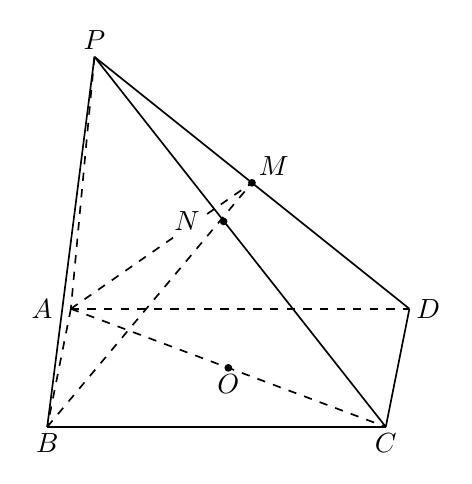
\begin{tikzpicture}[scale=1.0, semithick, every node/.style={inner sep=1.2pt}]
  \coordinate (A) at (2.60,3.40);
  \coordinate (B) at (2.30,1.90);
  \coordinate (C) at (6.60,1.90);
  \coordinate (D) at (6.90,3.40);
  \coordinate (P) at (2.90,6.60);
  \coordinate (O) at (4.60,2.65);
  \coordinate (M) at (4.90,5.00);
  \coordinate (N) at (4.54,4.51);

  % 可见棱
  \draw (P) -- (B);
  \draw (P) -- (C);
  \draw (P) -- (D);
  \draw (B) -- (C);
  \draw (C) -- (D);

  % 被遮挡的棱与辅助线
  \draw[dashed] (P) -- (A);
  \draw[dashed] (A) -- (B);
  \draw[dashed] (A) -- (D);
  \draw[dashed] (A) -- (C);
  \draw[dashed] (A) -- (M);
  \draw[dashed] (B) -- (M);

  \fill (M) circle (1.4pt);
  \fill (N) circle (1.4pt);
  \fill (O) circle (1.4pt);

  \node[above=1pt] at (P) {$P$};
  \node[left=5pt, fill=white, inner sep=1.4pt] at (A) {$A$};
  \node[below=1pt] at (B) {$B$};
  \node[below=1pt] at (C) {$C$};
  \node[right=1pt] at (D) {$D$};
  \node[above right=1pt] at (M) {$M$};
  \node[left=7pt, fill=white, inner sep=1.4pt] at (N) {$N$};
  \node[below=1pt] at (O) {$O$};
\end{tikzpicture}
